\chapter{Variability of AGN}
\label{chap:variability}
% 1.1 in Kara & Garcia

The first quasar discovered, 3C 273 \parencite{Edge19593C273Catalogue}, had been documented in photographic plates at least as early as 1887 \parencite{Slavchevamihova20133c273half}. This emblematic radio-loud object showed variable emission in the optical and radio bands on timescales from days to years \parencites{SmithH19633C273Var2}{Dent19653C273Var}, indicating that the size of the emitting region spanned only a few light-days in size. This compactness, coupled with the finding of its distant redshift \parencite{Schmidt19633C273z}, was very difficult to explain by dynamics that operate in normal galaxies, and variability thus became one of the key arguments that the enormous luminosities of quasars had to originate from an exceptionally compact and energetic central engine \parencites{Salpeter1964AccretionTheory}{Zeldovich1964AccretionTheory}.
% or some objects, rapid optical variability implied brightness temperatures that clearly required a nonthermal emission mechanism. For example, Oke (1967) observed day-to-day changes of 0.25 and 0.1 mag for 3C 279 and 3C 446 (Shields NED)

Now we know that variability in all wavelengths is an ubiquitous property of AGN, and so, its studies have been essential in understanding the physics of their nuclear regions, which, in general, cannot be resolved by current telescopes. This had been strictly true until the observations of Sgr A* and M87 \parencite{EventHorizonTelescope2019} and, more recently, with the GRAVITY interferometer on the VLT resolving the outer BLR in 3C 273 \parencite{Gravity20183C273BLR}; still, these surveys are limited to massive sources in the very nearby universe. 
For the vast majority of AGN, variability studies therefore rely on the \textit{light curve}, a time series recording how the brightness of the AGN, measured within a given wavelength band, varies over a monitoring period. The time scales, spectral changes, and the correlations and delays between variations extracted from these light curves provide crucial information on the nature and location of these components and on their interdependencies \parencite{Ulrich1997VARIABILITY}.

% Variability experiments mostly can be categorised by the region being probed and the type of \textit{reverberation signal} (\S \ref{ssec:RebMap}) being measured, as illustrated in Figure \ref{fig:CackettSchematic}. 
%\begin{figure}[t]
%    \centering
%    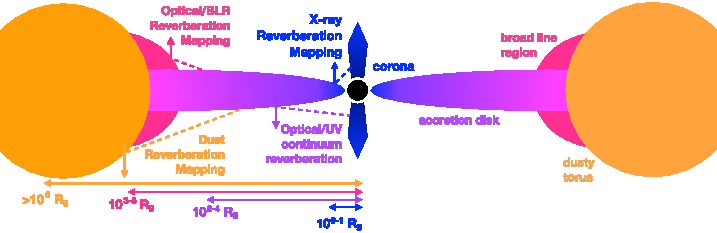
\includegraphics[width=\textwidth]{assets/2_figures/RM.pdf}
%    \caption[Schematic of AGN reverberation mapping across different physical scales]{\label{fig:CackettSchematic} Cross-sectional schematic of an AGN illustrating the four main types of reverberation mapping and their corresponding radial scales from the central black hole. Taken from \cite{Cackett2021RMFiguresGOOD}.}
%\end{figure}


\section{Physical Origin and Timescales}
\label{sec:PhysOrigin}

Early campaigns quickly revealed that AGN vary much more rapidly in X-rays than in the optical \parencite{WinklerWhite1975XRayVariab}, sometimes on timescales as short as a few minutes \parencite{McHardy1981minuteVar}, and that variability at different wavelengths is correlated \parencite{Ulrich1997VARIABILITY}. This stochastic behaviour can generally be explained by the \textit{propagating fluctuations} theory \parencite{Lyubarskii1997PropFluct}. Local fluctuations in the disk's surface density, presumably driven by the MRI (\S\,\ref{ssec:AccretionDisk}), occur at all radii and propagate inwards at the local viscous timescale\footnote{The viscous timescale, $t_\mathrm{visc} \sim r^2/\nu$, where $\nu$ is the kinematic viscosity, indicates the time for material to drift radially through the disk and increases with radius.}. As these fluctuations travel, they modulate the local mass accretion rate at progressively smaller radii, coupling the variability of the outer disk to that of the hotter inner regions and corona, where the shorter local viscous timescale drives faster fluctuations in the emitted luminosity \parencite{Uttley2023AccretionLags}. The X-ray variability produced in the innermost regions (i.e., in the corona) then irradiates the outer accretion disk and is reprocessed, driving the optical and UV variability observed at longer wavelengths with a characteristic time delay \parencite{Padovani2017whatisaname}, a \textit{reverberation}, as discussed below.
%Other mechanisms, including changes in line-of-sight obscuration, jet activity, or external perturbations like tidal disruption events (TDEs), can also contribute to the overall variability but are not described further here. 

Beyond this persistent stochastic variability, more extreme variability phenomena also exist, including \textit{changing-look} AGN, which undergo dramatic changes in their broad emission lines and continuum on timescales of months to years, possibly driven by rapid changes in accretion rate or obscuration \parencite{LaMassa2015ChangingLook}, as well as quasi-periodic eruptions (QPEs) and tidal disruption events (TDEs), they represent transient phenomena superimposed on the underlying stochastic variability and are not discussed further here.

%microvariability
Both propagating fluctuation lags and reverberation lags are simultaneously present in the data, but dominate at different temporal frequencies and have opposite energy dependences (Figure \ref{fig:KaraLags}). Fourier analysis allows the separation of both lag types into two temporal regimes: at low frequencies ($\nu \lesssim 10^{-5}$ Hz for a $10^6\,M_\odot$ black hole, or equivalently timescales $\gtrsim 1$ day), hard X-ray variations lag soft ones as accretion fluctuations propagate inward; at high frequencies ($\nu \gtrsim 10^{-3}$ Hz, timescales of minutes), soft X-rays lag hard ones as the disk responds to the driving corona \parencite{Kara2025SMBHXRayReview}. Simple cross-correlation averages over all timescales and can obscure this distinction, making Fourier analysis essential for disentangling the two contributions.

\begin{figure}[t]
    \centering
    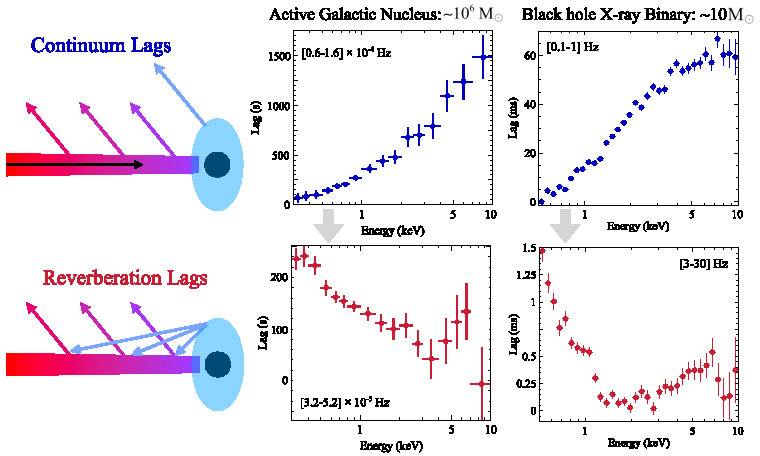
\includegraphics[width=\textwidth]{assets/2_figures/KaraLags.pdf}
    \caption[Continuum and reverberation lags as a function of energy and Fourier frequency]{\label{fig:KaraLags} Frequency-resolved X-ray time lags as a function of energy for an AGN ($\sim 10^6\,M_\odot$, left) and a black hole X-ray binary ($\sim 10\,M_\odot$, right), illustrating the universality of the two lag regimes. At low Fourier frequencies (top, blue), hard X-rays lag soft ones, consistent with inward-propagating accretion fluctuations. At high Fourier frequencies (bottom, red), soft X-rays lag hard ones, consistent with disk reverberation. Taken from \cite{Kara2025SMBHXRayReview}.}
\end{figure}

Variability-based methods are generally more effective than SED-based methods at identifying low-mass and low-luminosity AGN, since variability provides a cleaner signature of nuclear activity against the host galaxy background \parencite{YuEzTao2025}. Nonetheless, deriving the PSD/SF features and their uncertainties from an irregularly sampled light curve is very challenging, specially for stochastic light curves such as those of AGN; thereon, high quality light curves are indispensable to enable robust characterization of the UV/optical variability and interband lags \parencite{Kelly2014CARMA}.



\subsection{Reverberation Mapping}
\label{ssec:RebMap}

%ADD THE TF convolution Formula, limitations on different drivers yielfing same result and the lambda scaling of the time lags
Reverberation mapping (RM; \cite{Blandford1982RM}) exploits the fact that any region illuminated by the central engine responds to its variability with a characteristic lag $\tau = R/c$, where $R$ is the light travel distance to the responding region, providing a direct physical scale \parencite{Peterson2006BLR}. 

Formally, the observed emission-line light curve $L_l(t)$ is related to the driving continuum $L_c(t)$ through a convolution with the \textit{transfer function} $\Psi(\tau)$:


\begin{equation}
    \label{eq:TF}
    y(t) = \int_{-\infty}^{\infty} \Psi(\tau)\, y_{drive}(t - \tau)\, d\tau,
\end{equation}

where $\Psi(\tau)$ encodes the geometry and kinematics of the responding region \parencite{Netzer2013PhyEvolofAGNBook}. The centroid of $\Psi(\tau)$ gives the mean lag $\langle\tau\rangle$, and hence the characteristic size of the responding region. The characteristic timescales and size scales probed by different types of reverberation are summarised in Table \ref{tab:timescales} and Figure \ref{fig:CackettSchematic}.


\begin{figure}[t]
    \centering
    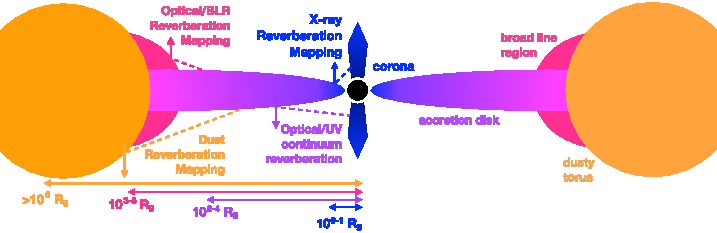
\includegraphics[width=\textwidth]{assets/2_figures/RM.pdf}
    \caption[Schematic of AGN reverberation mapping across different physical scales]{\label{fig:CackettSchematic} Cross-sectional schematic of an AGN illustrating the four main types of reverberation mapping and their corresponding radial scales from the central black hole. Taken from \cite{Cackett2021RMFiguresGOOD}.}
\end{figure}

 
\begin{table}[H]
\centering
\caption[AGN region size scales and variability timescales]{\label{tab:timescales} Order of magnitude size scales and their equivalent light-crossing times for the different regions of an AGN. Adapted from \cite{Cackett2021RMFiguresGOOD}.}
\begin{tabular}{lccc}
\hline%\hline
\noalign{\smallskip}
Region & Size scale & \multicolumn{2}{c}{Light-crossing time} \\
%\cline{3-4}
\noalign{\smallskip}
& ($R_g$) & $10^7\,M_\odot$ & $10^9\,M_\odot$ \\
\noalign{\smallskip}
\hline
\noalign{\smallskip}
X-ray corona    & $10$              & 500 s        & 14 hr        \\
UV/optical disk & $10^2$--$10^4$   & 0.06--6 days & 6--600 days  \\
BLR             & $10^3$--$10^5$   & 0.6--60 days & 60--6000 days\\
Dusty torus     & $>10^5$          & $>$60 days   & $>$6000 days \\
\noalign{\smallskip}
\hline
\end{tabular}
\end{table}


In the optical/UV, the most established application is BLR reverberation mapping, which measures the lag between continuum and broad emission line variations; since both the continuum and the broad lines are observed to vary in a correlated fashion, the measured lag directly yields the BLR size via $R_\mathrm{BLR} = c\tau$ \parencite{Peterson2006BLR}. As introduced in Section \ref{ssec:BLR}, this size scales with AGN luminosity as $R_\mathrm{BLR} \propto L^{1/2}$ \parencite{Kaspi2000BLRSScalingL}, a relationship empirically calibrated through RM campaigns % state that the relationship is for Hbeta and also is L_5000 etc
and used to estimate black hole masses via the virial theorem\footnote{$M_\mathrm{BH} = f R_\mathrm{BLR} \Delta V^2 / G$, where $\Delta V$ is the emission line width and $f$ is a geometric factor \parencite{Peterson2006BLR}.}. Continuum reverberation mapping instead measures the wavelength-dependent lags between different optical/UV bands, probing the accretion disk size and temperature profile. Under the standard irradiated disk model, the lag at wavelength $\lambda$ scales as \parencite{Netzer2022RM}:


\begin{equation}
    \label{eq:disklag}
    \tau_\lambda \propto \lambda^{4/3} \left[\frac{M_\mathrm{BH}\dot{M}}{(3 + f_\mathrm{irr})}\right]^{1/3},
\end{equation}

where $\dot{M}$ is the accretion rate and $f_\mathrm{irr}$ parameterizes the fraction of X-ray flux absorbed by the disk. This $\lambda^{4/3}$ scaling arises from the temperature profile of the standard thin disk ($T \propto r^{-3/4}$), with each wavelength probing emission from a characteristic disk radius. Observed continuum lags, however, are often larger than predicted by this simple model \parencite{Cackett2021RMFiguresGOOD}, partly because diffuse BLR emission contributes to the broadband continuum at larger radii than the disk itself, biasing the inferred lags towards longer values \parencites{Korista2001DiffusionContBLR}{Netzer2022RM}. Separating these contributions remains an active area of research, with microlensing studies offering an independent constraint on the disk size \parencite{Cackett2021RMFiguresGOOD}.

% but as might be expected, the response time of the disc to changes in Mdot does. 
% For example, disk models with alternative prescriptions for α, as well as the addition of a corona and jet, have been able to reproduce the variability of the microquasar GRS 1915+105 (Nayakshin et al. 2000; Janiuk et al. 2000, 2002). 
%Variability studies can therefore lend observational insight into the inadequacies of the traditional α prescription, and possibly lead to a more accurate characterization of the relationship between stress and pressure in the accretion disk. there has been discrepancies such as the ones calculated for the extra long lags and microlensing

%Observed continuum reverberation lags may be contaminated by diffuse BLR emission to the broadband continuum, which lies farther out in the accretion flow \parencites{Korista2001DiffusionContBLR}{Cackett2018DiffuseContBLR} and makes them appear longer than they really are.
%Variability-based methods are more effective than SED-based methods at identifying low mass and low luminosity AGN. % Cite Yu 2025 and references there in


\section{Variability Characterization}
\label{sec:VarChar}
Variability has been studied under a variety of methods, starting from simple statistical quantities tracing the amplitude and timescales of the observed variability to more sophisticated approaches in both the time and frequency domains \parencite{Paolillo2025Variability}. In general, these statistics attempt to measure the absolute or fractional variance of the light curve over some characteristic timescale $\Delta t$, or express the degree of correlation between different timescales or photometric bands \parencites{Ulrich1997VARIABILITY}{deCicco2025Variability}.

The distribution of variability power over temporal frequencies (or, equivalently, 1/timescale) is quantified by the \textit{power spectral density} (PSD), defined as the squared amplitude of the flux (e.g., \cite{Uttley2002PSD}). AGN PSDs typically follow a \quotes{red-noise} power law, $P(\nu) \propto \nu^{-\alpha}$ with $\alpha \sim 1$ at low frequencies, steepening to $\alpha \gtrsim 2$\footnote{$\alpha \sim 2$ corresponds to a \textit{Damped random walk} that breaks to flat slope at long timescales.} above a characteristic break frequency $\nu_b$, consequently displaying larger amplitude variations on longer timescales. This break timescale scales with black hole mass and accretion rate \parencite{McHardy2006Variab}, with smaller black holes varying more rapidly than larger ones for the same observing duration (Figure \ref{fig:KaraPSD}). The anticorrelation can be interpreted as a consequence of the fact that the most luminous AGN are likely to host larger mass black holes (if all quasars accrete at similar Eddington rates), in which case, their variability should be diluted by the larger emitting region \parencite{Paolillo2025Variability}. 

\begin{figure}[t]
    \centering
    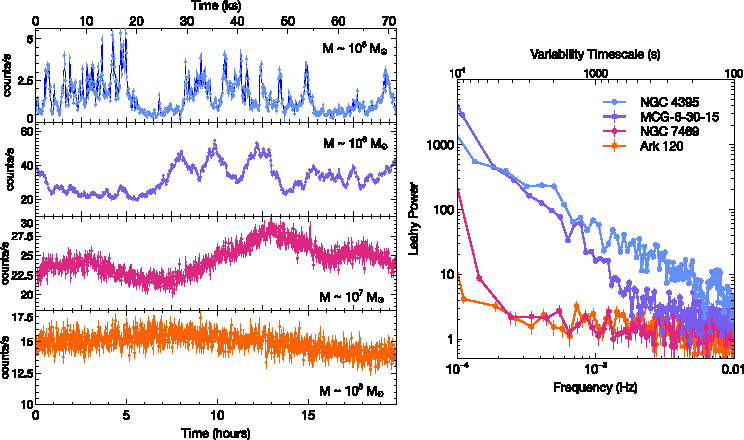
\includegraphics[width=1.0\textwidth]{assets/2_figures/KaraFig5.pdf}
    \caption[X-ray light curves and PSDs for four AGN spanning four decades in black hole mass]{\label{fig:KaraPSD} Left: X-ray light curves of four Seyfert~1 AGN with black hole masses spanning $10^5$--$10^8\,M_\odot$, observed with XMM-Newton over 70 ks. Smaller black holes vary more rapidly, with the $10^5\,M_\odot$ AGN (NGC 4395, top) showing variability on timescales of tens of seconds, while the $10^8\,M_\odot$ AGN (Ark 120, bottom) varies on timescales of hours. Right: The corresponding PSDs, showing the red-noise power-law shape characteristic of AGN X-ray variability. Taken from \cite{Kara2025SMBHXRayReview}.}
\end{figure}

The PSD also depends strongly on the observing waveband, with optical PSDs showing steeper slopes and lower normalization than X-ray PSDs, consistent with the propagating fluctuations picture where outer disk regions contribute power at lower frequencies and inner regions at higher ones \parencite{Kara2025SMBHXRayReview}.

A complementary time-domain characterization is provided by the \textit{structure function} (SF), which quantifies the mean variability amplitude as a function of time lag $\Delta t$; on short timescales the SF rises as a power law, flattening above a characteristic damping timescale $\tau$ that encodes the same physical information as the PSD break frequency \parencite{Kozlowski2016SF}.

% add this from Kelly 2014 sect. 1



% characteristic variability w/BH mass (Kara 3.3.1) and figures


%check Ricci for cHanging obscuration/state
%https://arxiv.org/pdf/2211.05132

%Check Faggin for current works 
%https://arxiv.org/abs/2410.18423

%PLOT: AGN classifications in the
%plane defined by the nuclear luminosity
%and variability 
%https://www.physik.uni-wuerzburg.de/fileadmin/11030400/Dissertation_Beuchert_Tobias.pdf


% check draganas lecture on:
% crossing times of different regions in the AGN (reb map)